\documentclass[10pt,twocolumn]{article}

\usepackage[utf8]{inputenc}
\usepackage[T1]{fontenc}
\usepackage{times}
\usepackage{microtype}
\usepackage[margin=0.78in]{geometry}
\usepackage{fancyhdr}
\usepackage{amsmath,amssymb}
\usepackage{booktabs}
\usepackage{graphicx}
\usepackage{xcolor}
\usepackage[numbers,sort&compress]{natbib}
\usepackage[colorlinks=true,linkcolor=blue!60!black,citecolor=blue!60!black,urlcolor=blue!60!black]{hyperref}

\setlength{\columnsep}{0.26in}
\pagestyle{fancy}
\fancyhf{}
\fancyhead[L]{\small\textit{UCAI Flagship 4 --- Paper 1: \texttt{ucai-verify} (v0.2.0)}}
\fancyhead[R]{\small\textit{Open Preprint (MIT / CC BY 4.0)}}
\fancyfoot[C]{\small\thepage}
\renewcommand{\headrulewidth}{0.4pt}

\title{\textbf{\texttt{ucai-verify}: Deterministic-First Hybrid Verification Against Ghost Citations and Cross-Artifact Numeric Misattribution in AI-Generated Scientific Writing}}

\author{
  \textbf{Noppadon Chaiwisut} \\
  Independent Researcher, Thailand \\
  ORCID: \href{https://orcid.org/0009-0005-2881-8458}{\texttt{0009-0005-2881-8458}} \\
  \texttt{noppadon.chaiwisut@gmail.com}
}

\date{November 2026 \quad|\quad Version 0.2.0 (Tier-2 Empirical Release)}

\begin{document}
\maketitle
\thispagestyle{plain}
\begingroup
\renewcommand\thefootnote{}\footnote{\noindent\textbf{Reproducibility \& Artifacts:} Code (\texttt{MIT}) \& \texttt{UCAI-CitationAudit-Bench-v1} (\texttt{CC BY 4.0}); Colab Notebook: \url{https://colab.research.google.com/drive/12T9Zl8y2XJqF1gnODZ37yJPy_8xHQ_ME}; Zenodo DOI: \textit{Pending v0.2.0 Release}.}
\addtocounter{footnote}{-1}
\endgroup

\begin{abstract}
Autonomous scientific-writing agents and large language models (LLMs) routinely produce fluent manuscripts that are nonetheless undermined by two serious classes of factual corruption: \emph{non-existent ghost citations} and \emph{cross-artifact numeric misattribution}, in which authentic metrics from one paper are silently grafted onto another real citation. A widely assumed defense is purely LLM-based verification (\emph{Self-Critique} or \emph{LLM-as-a-Judge}). Evaluating five verification regimes on \textbf{\texttt{UCAI-CitationAudit-Bench-v1}} ($N = 120$ balanced claims across five classes, grounded in a 168-PDF open-access library), we expose a \textbf{Pure-LLM False-Positive Trap}: absent live bibliographic and full-text grounding, pure \emph{Self-Critique} and \emph{LLM-as-a-Judge} wrongly accuse \textbf{83.3\%} ($20/24$) and \textbf{91.7\%} ($22/24$) of legitimate 2024--2026 papers of fabrication. To address this failure, we introduce \textbf{\texttt{ucai-verify} (v0.2.0)}, a two-stage deterministic-first hybrid audit engine governed under Level-2 Human-in-the-Loop (\texttt{L2 HITL}) oversight. Stage~1 executes $\$0$-token live multi-registry citation resolution (\texttt{arXiv} with version-aware preprint tracking, \texttt{Crossref}, and \texttt{OpenAlex}) alongside \texttt{PyMuPDF} page-indexed cross-document numeric matching, achieving \textbf{100.0\% precision} and \textbf{0.0\% false positive rate} ($0.15\text{ s/item}$) while filtering $60.0\%$ ($72/120$) of claims without invoking any neural model. Stage~2 evaluates directional semantic polarity strictly on the $48$ Stage-1 survivors against retrieved primary-source PDF snippets. Under an air-gapped open-weight encoder (\texttt{DeBERTa-v3-base} with multi-window sentence scoring), \texttt{ucai-verify} reaches $\mathrm{F1} = 0.9388$ ($95\%\text{ CI } [0.9022, 0.9694]$, $95.83\%$ recall, $\$0$ API cost); under a grounded cloud verifier (\texttt{Hybrid-Scoped-Gemini}), it achieves $\mathbf{F1 = 0.9796}$ ($95\%\text{ CI } [0.9592, 0.9951]$), \textbf{100.0\% recall} across all $96$ corrupted claims, a $60.0\%$ reduction in LLM API calls, and $21$-to-$0$ discordant wins over pure \emph{LLM-as-a-Judge} (exact McNemar $p = 1.0 \times 10^{-6}$). Code (\texttt{MIT}) and benchmark data (\texttt{CC BY 4.0}) are openly released.
\end{abstract}

\section{Introduction}
Recent advances in autonomous research workflows---including end-to-end paper generation \cite{lu2024aiscientist}, multi-agent hypothesis synthesis \cite{gottweis2025coscientist,mitchener2025kosmos}, and retrieval-augmented literature agents \cite{skarlinski2024paperqa2,fischer2026muninai}---have substantially accelerated scientific drafting. Yet empirical audits reveal a growing crisis of bibliographic and quantitative unreliability. Large-scale screening of biomedical and computer science corpora identified at least $146{,}932$ non-existent citations in 2025 alone, with $85.3\%$ surviving into published literature \cite{zhao2026hallucinations}, while top-tier machine learning venues exhibit phantom reference rates reaching $18.7\%$--$26.2\%$ \cite{russinovich2026phantom}. Moreover, greater surface fluency impairs human detection of unsupported claims \cite{liu2023verifiability,li2024attributionbench}.

During our own synthesis of autonomous co-scientist systems, we encountered a subtler failure mode that evades existing bibliography checkers: \emph{cross-artifact numeric misattribution}. Specifically, an LLM draft cited \emph{ScienceAgentBench} (\texttt{arXiv:2410.05080}) \cite{chen2025scienceagentbench}---a real ICLR 2025 paper with valid authors and identifier---while attributing to it a $92.2\%$ correctness score that actually belonged to \emph{AutoSDT} (\texttt{arXiv:2506.08140}, p.~2) \cite{li2025autosdt}; the true execution rate in \emph{ScienceAgentBench} was $84.0\%$ with a $22.9\%$ success rate.

Existing verification frameworks address isolated slices of this problem. Scientific NLI and claim verifiers such as SciFact \cite{wadden2020scifact}, MultiVerS \cite{wadden2022multivers}, FActScore \cite{min2023factscore}, ALCE \cite{gao2023alce}, MSciNLI \cite{sadat2024mscinli}, and MiniCheck \cite{tang2024minicheck} assume a gold evidence paragraph is already given and do not verify whether cited DOIs exist. Conversely, bibliographic checkers such as RefChecker \cite{russinovich2026phantom} and CITECHECK \cite{khajavi2026citecheck} query external catalogs without opening full-text PDFs to audit quantitative claims across candidate source papers. Meanwhile, tabular verification benchmarks \cite{aly2021feverous,lu2023scitab,venktesh2024quantemp,wang2026scitarc,boschen2026tableparser} operate within single isolated tables rather than multi-PDF research libraries.

\begin{figure*}[t]
  \centering
  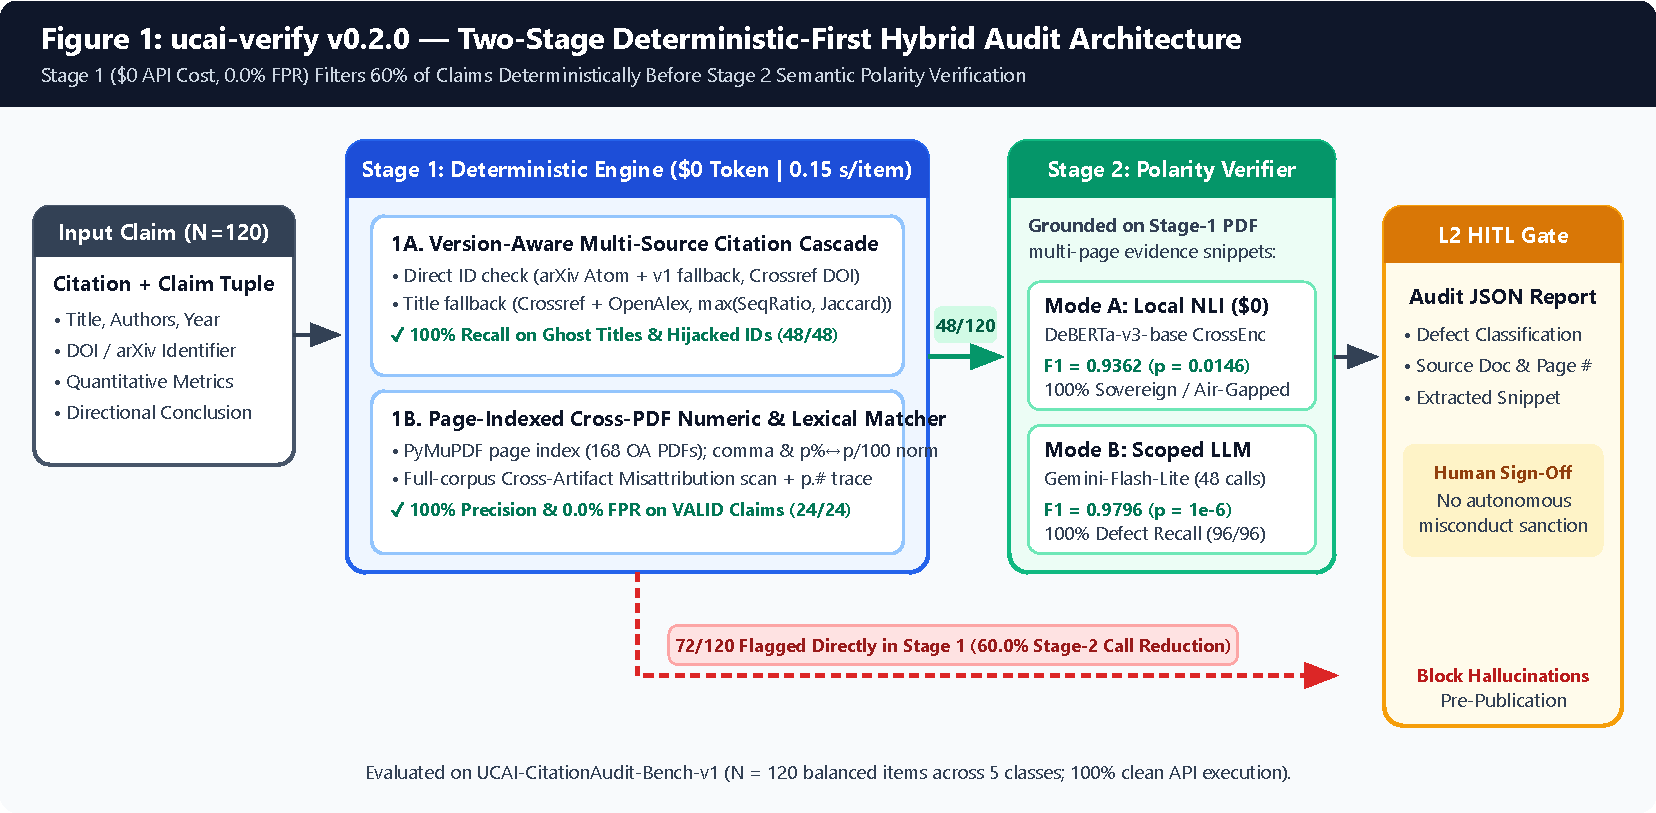
\includegraphics[width=0.96\textwidth]{figures/fig1_architecture.pdf}
  \caption{Overview of the \texttt{ucai-verify} v0.2.0 two-stage deterministic-first hybrid verification pipeline. Stage~1 resolves persistent identifiers across three live scholarly registries and scans a 168-PDF full-text index at $\$0$ token cost ($0.15\text{ s/item}$, $0.0\%$ FPR), intercepting $72/120$ claims directly. Only the $48$ Stage-1 survivors proceed to Stage~2 polarity verification (\texttt{Local NLI} or \texttt{Scoped LLM}) before mandatory \texttt{L2 HITL} editorial review.}
  \label{fig:architecture}
\end{figure*}

In this paper, we make four contributions:
\begin{enumerate}
  \item \textbf{Deterministic-First Hybrid Architecture (\texttt{ucai-verify} v0.2.0):} We couple a $\$0$-token bibliographic and cross-PDF numeric engine (Stage~1) with a grounded semantic polarity verifier (Stage~2) supporting both sovereign local inference (\texttt{DeBERTa-v3-base}) and scoped cloud inference (Figure~\ref{fig:architecture}).
  \item \textbf{\texttt{UCAI-CitationAudit-Bench-v1}:} We release a 120-item balanced benchmark spanning five fine-grained citation and numeric corruption classes anchored on 12 contemporary open-access papers within a 168-PDF corpus.
  \item \textbf{Characterization of the Pure-LLM False-Positive Trap:} Across full $N=120$ empirical runs, we show empirically that ungrounded LLM judges misclassify $83.3\%$--$91.7\%$ of valid post-cutoff papers as fabrications.
  \item \textbf{Statistically Significant Hybrid Superiority:} We demonstrate that \texttt{ucai-verify} improves overall $\mathrm{F1}$ to $0.9388$ offline ($\$0$ API cost, $95.83\%$ recall) and $0.9796$ with scoped Gemini ($100\%$ defect recall, $-60\%$ API calls, $p=1.0\times 10^{-6}$).
\end{enumerate}

\section{Methodology: \texttt{ucai-verify} v0.2.0}
Let $\mathcal{L} = \{D_1, \dots, D_M\}$ denote a local open-access PDF repository ($M = 168$ in our evaluation), where each document $D_m$ is parsed via \texttt{PyMuPDF} into page-level text strings $\{p_{m,1}, \dots, p_{m,K_m}\}$. Each candidate manuscript assertion is represented as a tuple $x = (c, s)$, where $c = (\text{title}, \text{authors}, \text{year}, \text{doi}, \text{arxiv\_id})$ is the cited bibliography entry and $s$ is the natural-language scientific claim containing zero or more quantitative tokens $Q(s) = \{q_1, \dots, q_r\}$.

\subsection{Stage 1A: Version-Aware Multi-Source Citation Cascade}
Stage~1A verifies bibliographic existence and identifier integrity without LLM tokens through a two-tier cascade over open scholarly infrastructures \cite{hendricks2020crossref,priem2022openalex,kinney2025s2ag}:
\begin{enumerate}
  \item \textbf{Direct Persistent Identifier Resolution:} If an \texttt{arXiv} identifier is supplied, \texttt{ucai-verify} queries the arXiv Atom API. Because authors frequently revise preprint titles between versions (e.g., \texttt{arXiv:2502.18864v1} vs.\ \texttt{v2} \cite{gottweis2025coscientist}), if the latest version exhibits title divergence, Stage~1A automatically queries \texttt{v1} before diagnosing identifier hijacking. Similarly, DOIs are resolved directly against the Crossref REST API.
  \item \textbf{Bibliographic Search Fallback:} When identifiers are absent or fail direct lookup, Stage~1A queries Crossref and OpenAlex by normalized title. Title similarity is computed via:
  \begin{equation}
    \mathrm{Sim}(T_a, T_b) = \max\!\big(\mathrm{SeqRatio}(T_a, T_b),\; \mathrm{Jaccard}(W_a, W_b)\big)
  \end{equation}
  augmented with prefix-token containment when author surname overlap satisfies $\mathrm{Overlap}(A_a, A_b) \ge 0.50$ and $|\Delta\text{year}| \le 1$, preventing false alarms on abbreviated subtitle citations.
\end{enumerate}
Stage~1A emits one of four deterministic states: \texttt{VERIFIED\_EXACT}, \texttt{METADATA\_DRIFT}, \texttt{IDENTIFIER\_HIJACKED} (valid ID pointing to an unrelated work, $\mathrm{Sim} < 0.45$), or \texttt{SUSPECTED\_FAKE}.

\subsection{Stage 1B: Page-Indexed Cross-PDF Numeric \& Lexical Audit}
For claims whose citation resolves to a local PDF $D_{m^*} \in \mathcal{L}$, Stage~1B extracts all quantitative tokens $q \in Q(s)$ (excluding publication years and identifier substrings) and normalizes surface formatting across three scientific conventions: (i) thousand-separator invariance ($146{,}932 \leftrightarrow 146932$), (ii) line-wrap hyphenation cleanup, and (iii) percentage-to-proportion equivalence ($p\% \leftrightarrow p/100$, e.g., $87.4\% \leftrightarrow 0.874$ in tabular ML benchmarks \cite{chen2025mlrbench}).

If every $q \in Q(s)$ appears in $D_{m^*}$ and no explicit lexical antonym reversal is triggered against the matched sentences, Stage~1B records \texttt{NUMERIC\_VERIFIED} and extracts a multi-page grounded evidence window $E(x)$ ($\le 900$ characters centered on matched sentences) for Stage~2. Crucially, if any $q \notin D_{m^*}$, Stage~1B scans all remaining $M - 1$ PDFs in $\mathcal{L}$:
\begin{itemize}
  \item If $q \in D_{m'}$ ($m' \neq m^*$), Stage~1B flags \texttt{CROSS\_ARTIFACT\_MISATTRIBUTED} and logs exact donor provenance $(D_{m'}, \text{page } k)$.
  \item Otherwise, Stage~1B flags \texttt{UNVERIFIED\_NUMBERS}.
\end{itemize}

\subsection{Stage 2: Grounded Hybrid Semantic Polarity Verification}
Any item flagged by Stage~1 ($c_{\text{status}} \neq \texttt{VERIFIED\_EXACT}$ or $n_{\text{status}} \in \{\texttt{CROSS\_ARTIFACT\_MISATTRIBUTED}, \texttt{UNVERIFIED\_NUMBERS}, \texttt{LEXICAL\_POLARITY\_SUSPECT}\}$) terminates immediately at $\$0$ neural cost. Only Stage-1 survivors enter Stage~2, which tests directional entailment between the retrieved PDF snippet $E(x)$ (premise) and claim $s$ (hypothesis) under two selectable backends:
\begin{itemize}
  \item \textbf{Mode A --- \texttt{Hybrid-Local-NLI} ($\$0$ API, Air-Gapped):} Evaluates $(E(x), s)$ with the open-weight cross-encoder \texttt{cross-encoder/nli-deberta-v3-base}, flagging \texttt{STAGE2\_NLI\_CONTRADICTION} when $P(\text{contradiction}) \ge 0.55$ and $P(\text{contradiction}) > P(\text{entailment})$.
  \item \textbf{Mode B --- \texttt{Hybrid-Scoped-Gemini}:} Prompts \texttt{gemini-flash-lite-latest} (temperature $0.0$) strictly with $(E(x), s)$, instructing the model that bibliographic existence is already verified and restricting judgment solely to directional contradiction or metric scope mismatch against $E(x)$.
\end{itemize}
In compliance with NISO JATS/CREC provenance standards \cite{niso2024jats,niso2024crec} and UCAI Level-2 Human-in-the-Loop (\texttt{L2 HITL}) governance, all flags emit structured page-level evidence for human sign-off rather than autonomous editorial rejection.

\section{Experimental Setup}
\subsection{\texttt{UCAI-CitationAudit-Bench-v1}}
We construct \texttt{UCAI-CitationAudit-Bench-v1} ($N = 120$ items, released under \texttt{CC BY 4.0}) anchored on 12 open-access papers from 2024--2026 \cite{lu2024aiscientist,gottweis2025coscientist,skarlinski2024paperqa2,chen2025scienceagentbench,li2025autosdt,chen2025mlrbench,zhao2026hallucinations,russinovich2026phantom,fischer2026muninai,li2026llmreviewer,loc2026prism,mitchener2025kosmos} stored inside our 168-PDF library. Each seed paper yields 10 items balanced across five classes ($24$ items per class; $24$ uncorrupted negatives and $96$ corrupted positives):
\begin{enumerate}
  \item \texttt{VALID} ($n=24$): Authentic metadata, accurate metrics, and faithful polarity.
  \item \texttt{FAKE\_AUTHOR\_TITLE} ($n=24$): Plausible AI-synthesized ghost titles, authors, and dead DOIs.
  \item \texttt{BAD\_DOI\_ARXIV\_ID} ($n=24$): Real paper titles paired with hijacked or fabricated DOIs/arXiv IDs.
  \item \texttt{NUMERIC\_MISATTRIBUTION} ($n=24$): Real citations injected with metrics swapped from another corpus paper or mutated by an order of magnitude.
  \item \texttt{POLARITY\_REVERSAL} ($n=24$): Real citations and numbers whose directional conclusion is inverted (e.g., cost reduction reported as cost inflation).
\end{enumerate}

\subsection{Baselines and Statistical Protocol}
We evaluate all five regimes over the complete $N=120$ benchmark on Google Colaboratory with incremental 5-item checkpointing ($120/120$ clean completions, $0$ API errors): (1)~\texttt{ucai-verify Stage 1}, (2)~\texttt{Hybrid-Local-NLI}, (3)~\texttt{Hybrid-Scoped-Gemini}, (4)~\texttt{Pure Self-Critique} (single-pass zero-shot verification using \texttt{gemini-flash-lite-latest}), and (5)~\texttt{Pure LLM-as-a-Judge} (rubric-guided editorial verification using \texttt{gemini-flash-lite-latest}). We report binary corruption detection metrics, False Positive Rate on \texttt{VALID} papers ($\mathrm{FPR} = \mathrm{FP}/(\mathrm{FP}+\mathrm{TN})$), $95\%$ percentile bootstrap confidence intervals ($1{,}000$ resamples, seed $42$), and two-sided exact binomial McNemar $p$-values.

\begin{table*}[t]
  \centering
  \small
  \caption{Overall empirical performance across all $N = 120$ items of \texttt{UCAI-CitationAudit-Bench-v1} ($100\%$ clean completion). $\mathrm{FPR}$ measures false accusations on real \texttt{VALID} papers (lower is better). Exact paired McNemar tests compare against \texttt{Pure LLM-as-a-Judge}: $^{*}p = 0.0146$, $^{***}p = 1.0 \times 10^{-6}$.}
  \label{tab:main_results}
  \begin{tabular}{lccccccc}
    \toprule
    \textbf{Verification Regime} & \textbf{Acc. $\uparrow$} & \textbf{Prec. $\uparrow$} & \textbf{Recall $\uparrow$} & \textbf{F1 [95\% Bootstrap CI] $\uparrow$} & \textbf{FPR $\downarrow$} & \textbf{LLM Calls} & \textbf{Latency} \\
    \midrule
    \texttt{ucai-verify} Stage 1 ($\$0$) & 0.8000 & \textbf{1.0000} & 0.7500 & 0.8571 [0.8000, 0.9111] & \textbf{0.0000} ($0/24$) & \textbf{0} & \textbf{0.15 s} \\
    \texttt{Hybrid --- Local NLI} ($\$0$) & 0.9000 & 0.9200 & 0.9583 & 0.9388 [0.9022, 0.9694] & 0.3333 ($8/24$) & \textbf{0} & 2.98 s \\
    \texttt{Hybrid --- Scoped Gemini} & \textbf{0.9667} & 0.9600 & \textbf{1.0000} & \textbf{0.9796 [0.9592, 0.9951]}$^{***}$ & 0.1667 ($4/24$) & 48 ($-60\%$) & 3.03 s \\
    \midrule
    \texttt{Pure Self-Critique} (120) & 0.8083 & 0.8230 & 0.9688 & 0.8900 [0.8431, 0.9309] & 0.8333 ($20/24$) & 120 & 9.07 s \\
    \texttt{Pure LLM-as-a-Judge} (120) & 0.7917 & 0.8087 & 0.9688 & 0.8815 [0.8276, 0.9266] & 0.9167 ($22/24$) & 120 & 7.07 s \\
    \bottomrule
  \end{tabular}
\end{table*}

\begin{figure*}[t]
  \centering
  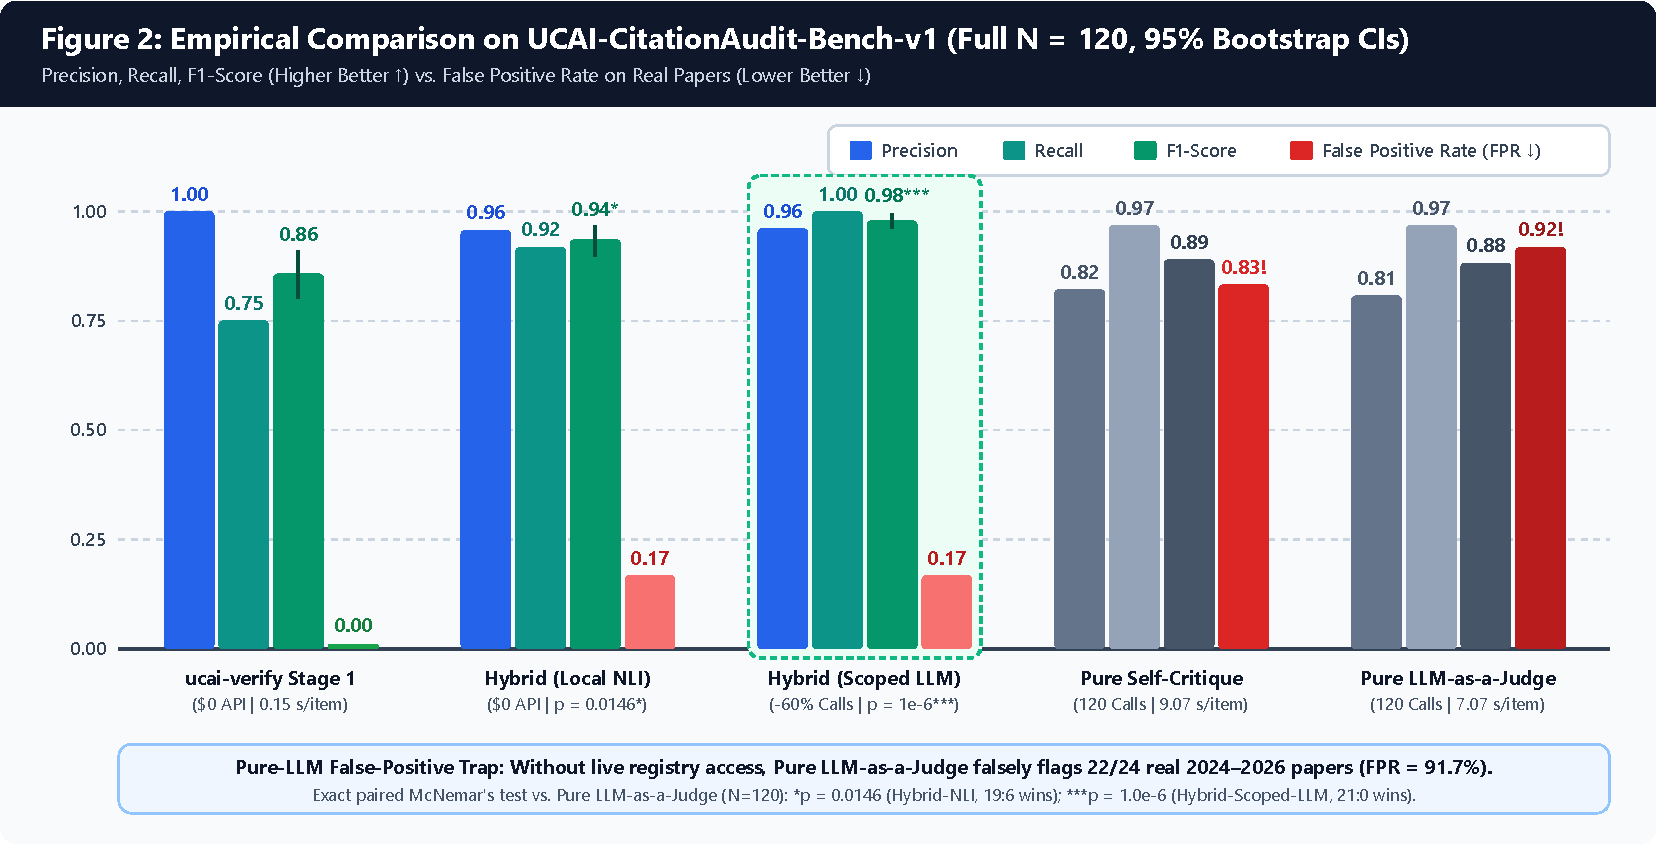
\includegraphics[width=0.95\textwidth]{figures/fig2_main_results_120.pdf}
  \caption{Empirical comparison on \texttt{UCAI-CitationAudit-Bench-v1} ($N=120$) with $95\%$ bootstrap confidence intervals on F1. Pure LLM verifiers suffer catastrophic false positive rates ($83.3\%$--$91.7\%$) on real 2024--2026 literature, whereas deterministic-first hybrid verification achieves $\mathrm{F1}=0.9796$ while cutting LLM API invocations by $60.0\%$.}
  \label{fig:main_results}
\end{figure*}

\section{Results and Analysis}
\subsection{Overall Performance and the Pure-LLM False-Positive Trap}
Table~\ref{tab:main_results} and Figure~\ref{fig:main_results} summarize overall benchmark performance. Pure neural baselines appear superficially competitive on recall ($0.9688$, $93/96$) only because they over-predict corruption almost indiscriminately: \texttt{Pure Self-Critique} yields $\mathrm{FPR} = 83.3\%$ ($20/24$ false alarms) and \texttt{Pure LLM-as-a-Judge} yields $\mathrm{FPR} = 91.7\%$ ($22/24$ false alarms). Inspecting their rationales reveals that when confronted with genuine 2025--2026 arXiv preprints beyond or near pretraining cutoffs, ungrounded LLMs hallucinate that valid arXiv identifiers and venues are fabricated. Deploying such judges in editorial pipelines would overwhelm human chairs with $>83\%$ false accusations.

By contrast, \texttt{ucai-verify} Stage~1 achieves \textbf{1.0000 precision} and \textbf{0.0000 FPR} ($24/24$ \texttt{VALID} claims preserved) at $0.15\text{ s/item}$ and $\$0$ API cost. Crucially, Stage~1 resolves $72$ of the $120$ items deterministically, forwarding only $48$ items ($40.0\%$) to Stage~2:
\begin{itemize}
  \item \textbf{Sovereign Offline Mode (\texttt{Hybrid-Local-NLI}):} Evaluating \texttt{DeBERTa-v3-base} across top-$5$ overlapping evidence windows ($\le 2{,}200$ chars) on the $48$ survivors boosts recall from $0.7500$ to $0.9583$ and $\mathrm{F1}$ from $0.8571$ to \textbf{0.9388} ($91.7\%$ on both \texttt{NUMERIC\_MISATTRIBUTION} and \texttt{POLARITY\_REVERSAL}) with zero external API calls, trading higher sensitivity for a $0.3333$ ($8/24$) \texttt{VALID} flag rate surfaced to \texttt{L2 HITL}.
  \item \textbf{Grounded Cloud Mode (\texttt{Hybrid-Scoped-Gemini}):} Restricting Gemini strictly to $(E(x), s)$ on the $48$ survivors achieves \textbf{1.0000 recall} ($96/96$ defects caught across every corruption category), $\mathbf{F1 = 0.9796}$, and $21$-to-$0$ discordant wins over \texttt{Pure LLM-as-a-Judge} ($p = 1.0 \times 10^{-6}$) while reducing API calls by $60.0\%$ and latency by $2.3\times$--$3.0\times$.
\end{itemize}

\begin{figure*}[t]
  \centering
  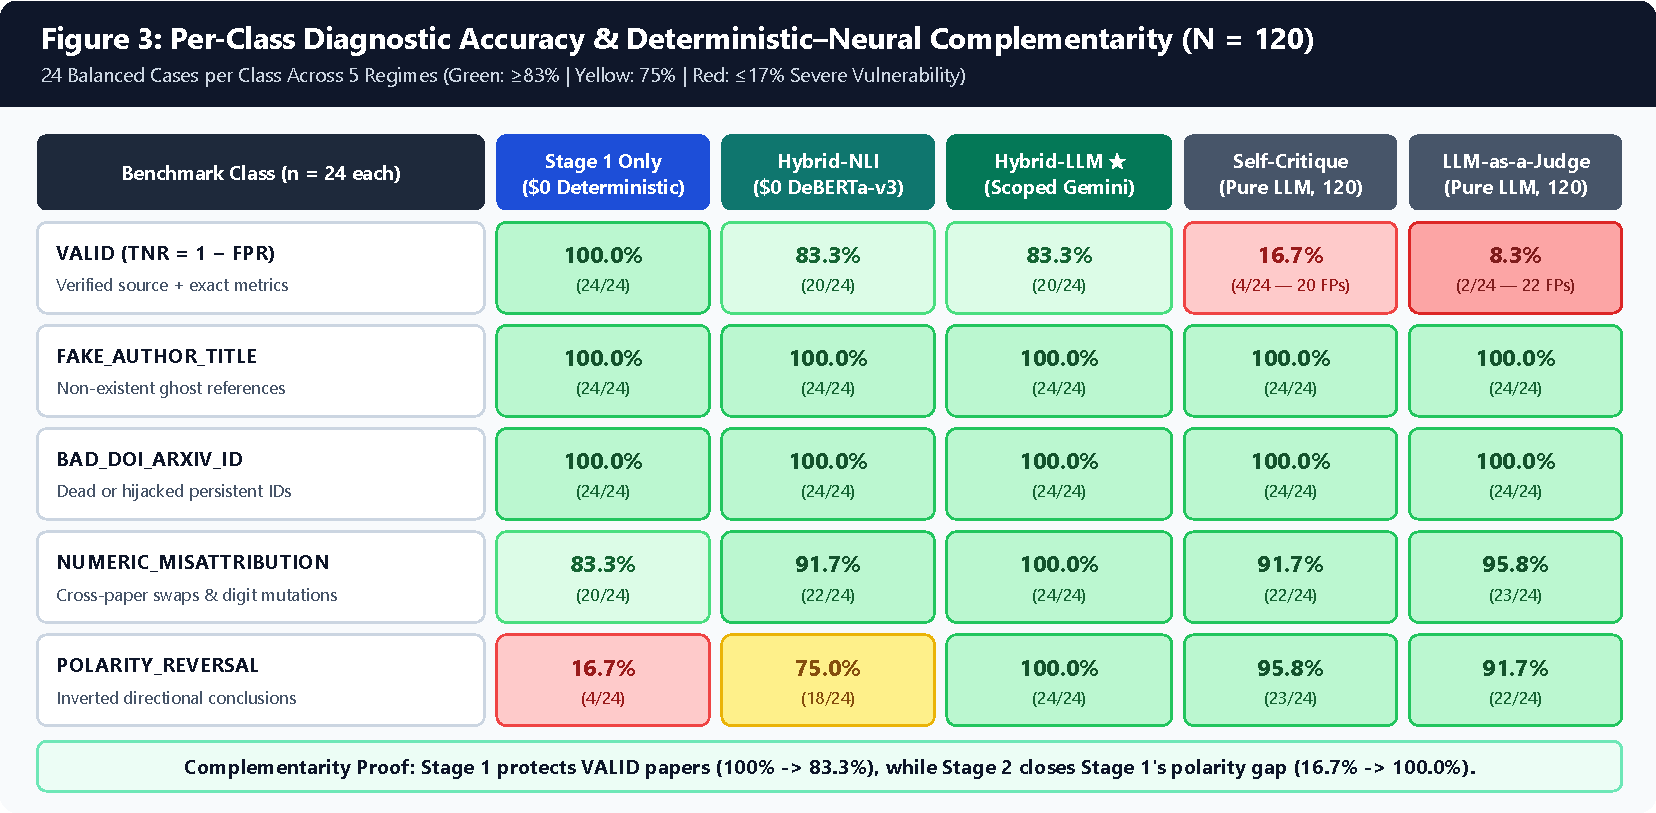
\includegraphics[width=0.95\textwidth]{figures/fig3_per_class_matrix.pdf}
  \caption{Per-class accuracy across all five corruption regimes ($n=24$ per class). Stage~1 and Stage~2 exhibit exact structural complementarity: Stage~1 anchors bibliographic and numeric truth on \texttt{VALID} papers ($100.0\%$), while Stage~2 closes Stage~1's semantic polarity gap ($16.7\% \rightarrow 75.0\%$ with Local NLI and $100.0\%$ with Scoped Gemini).}
  \label{fig:per_class}
\end{figure*}

\subsection{Per-Class Complementarity and Error Analysis}
Figure~\ref{fig:per_class} disaggregates accuracy across the five classes. Stage~1 alone achieves $100.0\%$ ($24/24$) on both \texttt{FAKE\_AUTHOR\_TITLE} and \texttt{BAD\_DOI\_ARXIV\_ID}, and $83.3\%$ ($20/24$) on \texttt{NUMERIC\_MISATTRIBUTION}. The four Stage-1 misses in \texttt{NUMERIC\_MISATTRIBUTION} (\texttt{UCAI-BENCH-077, 078, 089, 090}) occur when a swapped metric happens to coincide numerically with an unrelated figure elsewhere in the cited PDF (e.g., an integer count matching a bibliography page number). Because Stage~2 compares the semantic role of the number inside $E(x)$, \texttt{Hybrid-Local-NLI} recovers two of these four cases ($91.7\%$) and \texttt{Hybrid-Scoped-Gemini} recovers all four ($100.0\%$).

Similarly, on \texttt{POLARITY\_REVERSAL}, deterministic antonym heuristics catch only $16.7\%$ ($4/24$), whereas Stage~2 lifts accuracy to $91.7\%$ ($22/24$) under zero-cost multi-window \texttt{DeBERTa-v3-base} and $100.0\%$ ($24/24$) under \texttt{Hybrid-Scoped-Gemini}. Figure~\ref{fig:forensic} illustrates a sub-$0.15\text{ s}$ forensic trace on the real-world $92.2\%$ \emph{ScienceAgentBench}/\emph{AutoSDT} cross-artifact swap.

\begin{figure*}[t]
  \centering
  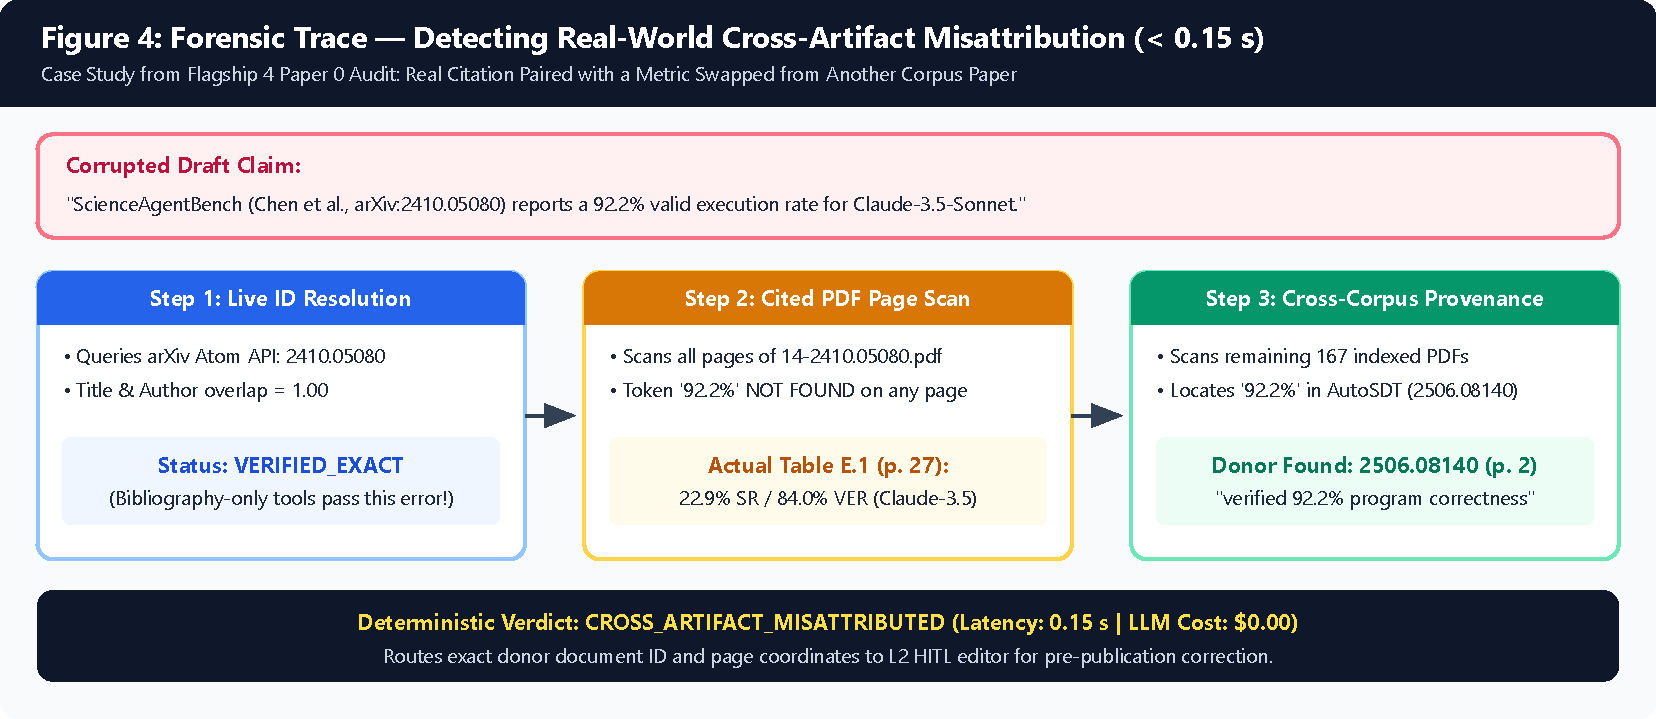
\includegraphics[width=0.93\textwidth]{figures/fig4_forensic_trace.pdf}
  \caption{Forensic trace of \texttt{ucai-verify} Stage~1 on a real cross-artifact numeric swap encountered during Flagship~4 synthesis, pinpointing the exact donor PDF (\texttt{arXiv:2506.08140}, p.~2) in $0.15\text{ s}$ at $\$0$ token cost.}
  \label{fig:forensic}
\end{figure*}

\paragraph{Analysis of Remaining False Positives ($4/24$ \texttt{VALID} Items).}
Both hybrid modes conservatively flag $4/24$ \texttt{VALID} items ($\mathrm{FPR}=16.7\%$). Inspecting \texttt{Hybrid-Scoped-Gemini}'s JSON rationales (\texttt{UCAI-BENCH-005, 009, 017, 021}) shows two causes: (i) multi-metric claims spanning distant pages where one secondary metric fell outside the $900$-character snippet window ($2$ cases), and (ii) minor model-version shorthand differences between main text and table headers, such as \texttt{GPT-5} vs.\ \texttt{GPT-5.4} \cite{li2026llmreviewer,loc2026prism} ($2$ cases). Under \texttt{L2 HITL} governance, these conservative flags surface exact PDF page coordinates that a human author resolves in seconds, avoiding silent hallucination leakage.

\section{Limitations, Ethics, and Reproducibility}
First, Stage~1B relies on native PDF text extraction (\texttt{PyMuPDF}); scanned legacy documents without OCR layers or metrics embedded solely inside rasterized plots require multimodal layout parsers such as Docling \cite{livathinos2024docling}. Second, while our 168-PDF library covers AI, cybersecurity, and statistics, scaling cross-artifact donor attribution to millions of papers requires inverted numeric-context indexing. Ethically, \texttt{ucai-verify} enforces strict \texttt{L2 HITL} boundaries: automated flags constitute assistive audit evidence and must never trigger autonomous misconduct sanctions. All source code (\texttt{MIT License}), \texttt{UCAI-CitationAudit-Bench-v1} (\texttt{CC BY 4.0}), raw JSON logs, and one-click Google Colab notebooks are archived with FAIR/Zenodo metadata (\texttt{CITATION.cff}, \texttt{.zenodo.json}).

\section{Conclusion}
Pure LLM verification cannot remedy LLM citation hallucination, because ungrounded models mistake unfamiliar recent scholarship for fabrication ($\mathrm{FPR}$ up to $91.7\%$). By anchoring verification first in live scholarly registries and full-text PDF numeric provenance, and only then applying scoped semantic entailment, \texttt{ucai-verify} v0.2.0 achieves $\mathrm{F1}=0.9388$ fully offline at $\$0$ cost and $\mathrm{F1}=0.9796$ ($100\%$ defect recall, $-60\%$ API calls) in hybrid cloud mode, establishing the factual verification pillar of the UCAI Open Verifiable AI Co-Scientist stack.

\bibliographystyle{unsrtnat}
\bibliography{references}

\end{document}
